\documentclass{standalone}

% graphics
\usepackage{tikz}
\usepackage{pgfplots}
\usepackage{siunitx}

\begin{document}

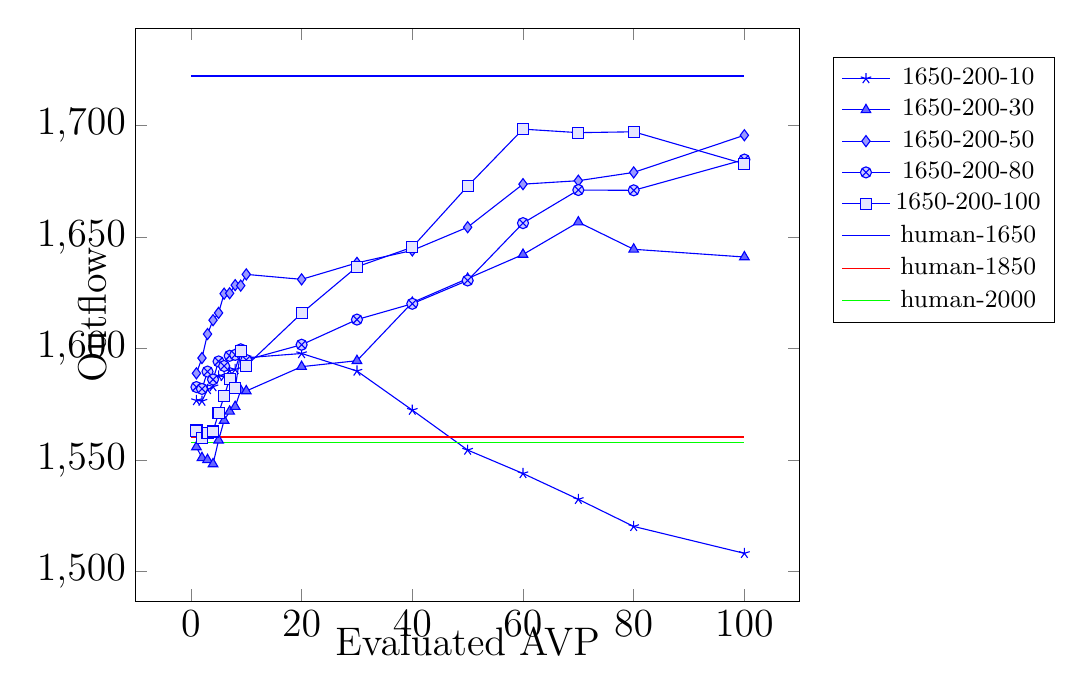
\begin{tikzpicture}[scale=1]
  \pgfplotsset{
      scale only axis,
      every x tick label/.append style={font=\Large},
      every y tick label/.append style={font=\Large},
	legend style={at={(1.05,0.95)},anchor=north west}
  }

\pgfplotscreateplotcyclelist{mycolorlist}{%
	blue,every mark/.append style={fill=blue!80}, mark=star, error bars/.cd, y dir=both, y explicit\\%
	blue,every mark/.append style={fill=blue!60}, mark=triangle*, error bars/.cd, y dir=both, y explicit\\%
	blue,every mark/.append style={fill=blue!40}, mark=diamond*, error bars/.cd, y dir=both, y explicit\\%
	blue,every mark/.append style={fill=blue!20}, mark=otimes*, error bars/.cd, y dir=both, y explicit\\%
	blue,every mark/.append style={fill=blue!10}, mark=square*, error bars/.cd, y dir=both, y explicit\\%
	red,densely dashed,every mark/.append style={solid,fill=red!80}, mark=star, error bars/.cd, y dir=both, y explicit\\%
	red,densely dashed,every mark/.append style={solid,fill=red!60},mark=triangle*, error bars/.cd, y dir=both, y explicit\\%
	red,densely dashed,every mark/.append style={solid,fill=red!40},mark=diamond*, error bars/.cd, y dir=both, y explicit\\%
	red,densely dashed,every mark/.append style={solid,fill=red!20}, mark=otimes*, error bars/.cd, y dir=both, y explicit\\%
	red,densely dashed,every mark/.append style={solid,fill=red!10}, mark=square*, error bars/.cd, y dir=both, y explicit\\%
	green!40!black, dashed,every mark/.append style={solid,fill=green!80}, mark=star, error bars/.cd, y dir=both, y explicit\\%
	green!40!black, dashed,every mark/.append style={solid,fill=green!60},mark=triangle*, error bars/.cd, y dir=both, y explicit\\%
	green!40!black, dashed,every mark/.append style={solid,fill=green!40},mark=diamond*, error bars/.cd, y dir=both, y explicit\\%
	green!40!black, dashed,every mark/.append style={solid,fill=green!20},mark=otimes*, error bars/.cd, y dir=both, y explicit\\%
	green!40!black, dashed,every mark/.append style={solid,fill=green!10},mark=square*, error bars/.cd, y dir=both, y explicit\\%
	black, dashed,every mark/.append style={solid,fill=green!80}, mark=star, error bars/.cd, y dir=both, y explicit\\%
	black, dashed,every mark/.append style={solid,fill=green!60},mark=triangle*, error bars/.cd, y dir=both, y explicit\\%
	black, dashed,every mark/.append style={solid,fill=green!40},mark=diamond*, error bars/.cd, y dir=both, y explicit\\%
	black, dashed,every mark/.append style={solid,fill=green!20},mark=otimes*, error bars/.cd, y dir=both, y explicit\\%
	black, dashed,every mark/.append style={solid,fill=green!10},mark=square*, error bars/.cd, y dir=both, y explicit\\%
	}


\begin{axis}[
    legend style={font=\small},
	ylabel={\Large Outflow},
	x label style={at={(axis description cs:0.5,-0.03)},anchor=north},
	y label style={at={(axis description cs:-0.030,0.5)}, anchor=south},
	xlabel={\Large Evaluated AVP},
	cycle list name=mycolorlist
]

\addplot table [x=a, y=b] {
a	 b	 c
1	1576.76	28.39
2	1576.48	25.88
3	1581.7	29.78
4	1582.96	31.9
5	1587.74	32.32
6	1587.53	30.75
7	1590.08	31.5
8	1590.66	30.57
9	1598.22	30.1
10	1595.92	26.3
20	1597.82	33.57
30	1589.98	37.02
40	1572.44	38.65
50	1554.55	37.2
60	1544.04	40.9
70	1532.48	38.11
80	1520.32	36.95
100	1508.26	46.41
};
\label{1650-200-10}

\addplot table [x=a, y=b] {
a	 b	 c
1	1555.92	39.32
2	1551.06	40.12
3	1550.16	42.57
4	1548.32	51.54
5	1558.94	47.67
6	1567.8	54.85
7	1571.87	49.57
8	1573.99	49.79
9	1581.3	48.58
10	1581.01	45.14
20	1591.92	59.26
30	1594.58	57.9
40	1620.65	61.36
50	1631.41	64.86
60	1642.18	57.45
70	1656.68	68.61
80	1644.52	72.62
100	1641.06	78.52
};
\label{1650-200-30}

\addplot table [x=a, y=b] {
a	 b	 c
1	1588.93	31.15
2	1595.77	28.75
3	1606.54	32.06
4	1612.76	35.62
5	1616.0	36.1
6	1624.64	35.64
7	1624.82	34.65
8	1628.46	31.19
9	1628.24	36.06
10	1633.28	36.46
20	1631.05	48.84
30	1638.43	53.33
40	1644.01	59.42
50	1654.42	56.11
60	1673.71	61.74
70	1675.26	63.79
80	1678.97	60.94
100	1695.64	52.32
};
\label{1650-200-50}

\addplot table [x=a, y=b] {
a	 b	 c
1	1582.78	29.71
2	1581.95	29.38
3	1589.72	30.36
4	1586.16	32.28
5	1594.26	34.23
6	1592.21	33.52
7	1596.78	33.07
8	1597.21	35.79
9	1599.7	35.97
10	1594.94	35.13
20	1601.75	39.31
30	1613.02	49.56
40	1620.11	51.64
50	1630.55	52.0
60	1656.25	58.97
70	1671.08	51.89
80	1670.94	52.84
100	1684.73	41.24
};
\label{1650-200-80}

\addplot table [x=a, y=b] {
a	 b	 c
1	1563.3	33.96
2	1559.77	36.13
3	1562.15	41.08
4	1562.87	44.46
5	1571.11	42.3
6	1578.6	45.84
7	1586.45	42.79
8	1582.2	45.92
9	1598.83	41.57
10	1592.28	35.67
20	1615.86	42.48
30	1636.67	49.27
40	1645.45	52.19
50	1672.78	54.33
60	1698.37	51.23
70	1696.79	45.27
80	1697.18	37.9
100	1682.78	35.17
};
\label{1650-200-100}

\addplot[blue, samples=200] coordinates {(0,1722.200000) (100,1722.200000)};\label{human-1650}\addplot[red, samples=200] coordinates {(0,1560.380000) (100,1560.380000)};\label{human-1850}\addplot[green, samples=200] coordinates {(0,1558.120000) (100,1558.120000)};\label{human-2000}\addlegendimage{/pgfplots/refstyle=1650-200-10}
\addlegendentry{1650-200-10}
\addlegendimage{/pgfplots/refstyle=1650-200-30}
\addlegendentry{1650-200-30}
\addlegendimage{/pgfplots/refstyle=1650-200-50}
\addlegendentry{1650-200-50}
\addlegendimage{/pgfplots/refstyle=1650-200-80}
\addlegendentry{1650-200-80}
\addlegendimage{/pgfplots/refstyle=1650-200-100}
\addlegendentry{1650-200-100}
\addlegendimage{/pgfplots/refstyle=human-1650}
\addlegendentry{human-1650}
\addlegendimage{/pgfplots/refstyle=human-1850}
\addlegendentry{human-1850}
\addlegendimage{/pgfplots/refstyle=human-2000}
\addlegendentry{human-2000}


\end{axis}
\end{tikzpicture}
\end{document}
